% !TeX root = blatt05.tex

%----------------------------------------------------------------%
%--------------------------GRUNDEINSTELLUNGEN--------------------%
%----------------------------------------------------------------%
\documentclass[oneside, ngerman, footinclude=off, captions=tableheading]{scrartcl}
%	'oneside'/'twoside': nicht zwischen linker und rechter Seite unterscheiden (alternativ twoside)
%	'twocolumn': wuerde 2 Spalten auf dem Blatt platzieren
%	'bibliography=totocnumbered': Normal nummeriertes Inhaltsverzeichnis (Kapitelnummer)
%	'listof=totocnumbered': Abbildungs- und Tabellenverzeichnis normal nummeriert (Kapitelnummer)
%	'ngerman' verwendet deutsch als Dokumentensprache (z.B. fuer Sirange)
%	'footinclude=off': Zaehlt Fusszeile zum Rand (vergroessert den Textbereich)
%	'captions=tableheading': Tabellenueberschriften explizit verwenden, erhoeht den Abstand zur Tabelle

\usepackage[ngerman]{babel}		%	Einstellen der Sprache
\usepackage[T1]{fontenc}		%	Wie wird Text ausgegeben, d.h. im PDF
\usepackage[utf8]{inputenc}		%	Welche Zeichen 'versteht' LaTeX bei der Eingabe?
\usepackage{lmodern}			%	Laedt Schriften, die geglaettet sind
\usepackage{blindtext}			%	Beispieltext, zum Testen geeignet

%----------------------------------------------------------------%
%--------------------------ABSTÄNDE------------------------------%
%----------------------------------------------------------------%
%\usepackage[onehalfspacing]{setspace}				%	Für Zeilenabstaende: 'singlespacing' (einfach), 'onehalfspacing' (1.5-fach), 'doublespacing' (2fach)
%\setlength{\parindent}{0cm}						%	Laengenangabe für die Einrueckung der ersten Zeile eines neuen Absatzes.
%\setlength{\parskip}{6pt plus 3pt minus 3pt}		%	Laengenangabe für den Abstand zwischen zwei Absaetzen.
%	Wenn diese beiden Befehle nicht kommentiert sind, wird ein Absatz nicht eingezogen sondern es gibt einen Abstand

% kleinere Abstände über und unter Gleichungen
\usepackage{setspace}\onehalfspacing
\AtBeginDocument{%
  \addtolength\abovedisplayskip{-0.2\baselineskip}
  \addtolength\belowdisplayskip{-0.2\baselineskip}
}

%----------------------------------------------------------------%
%--------------------------MATHE---------------------------------%
%----------------------------------------------------------------%
\usepackage[]{mathtools}							%	Erweiterung von AMSMath, laedt automatisch AMSMath - für viele Mathe-Werkzeuge, 'fleqn' als Option ist für Mathe linksbuendig
\usepackage{amsfonts}								%	Für eine Vielzahl an mathematischen Symbolen
\usepackage{nicefrac}

%----------------------------------------------------------------%
%--------------------------KOPF- UND FUSSZEILEN------------------%
%----------------------------------------------------------------%
\usepackage[automark,headsepline=.4pt]{scrlayer-scrpage}
\pagestyle{scrheadings}
\setkomafont{pageheadfoot}{\normalfont\bfseries}	%	Normale Schriftart und Fett für den Seitenkopf
\addtokomafont{pagenumber}{\normalfont\bfseries}	%	Normale Schriftart und Fett für die Seitenzahl
\clearpairofpagestyles								%	Löscht die Seitenkopf- und Seitenzahlen
\ohead{\thepage}									%	Rechter Seitenkopf mit Seitenzahl
\ihead{\headmark}									%	Linker Seitenkopf mit section
\ofoot[]{\empty}									%	Leere Fußzeile, ungerade Seiten
%	Definert man oben in der documentclass 'twoside', so wird zwischen geraden und ungeraden Seiten unterschieden (NUR DANN!)

%----------------------------------------------------------------%
%--------------------------BILDER--------------------------------%
%----------------------------------------------------------------%
\usepackage{graphicx}									%	Um Bilder einbinden zu koennen 
\usepackage[dvipsnames,svgnames,table]{xcolor}			%	Farben verwenden, Versch. Farbdefinitionen, Farben in Tabellen (-Reihen, -Spalten)
\usepackage{pdfpages}									%	pdfs importieren
\definecolor{Seeblau100}{RGB}{0,169,224}				%	Uni-Farben, z.B. fuer Tabellen
\definecolor{Seeblau65}{RGB}{89,199,254}
\definecolor{Seeblau35}{RGB}{165,224,254}
\definecolor{Seeblau20}{RGB}{203,237,254}
\definecolor{Seegrau60}{RGB}{102,102,102}
\definecolor{Seegrau40}{RGB}{153,153,153}
\definecolor{Seegrau20}{RGB}{204,204,204}
\definecolor{Seegrau10}{RGB}{230,230,230}

%----------------------------------------------------------------%
%--------------------------POSITIONIERUNG------------------------%
%----------------------------------------------------------------%
\usepackage{float}

%----------------------------------------------------------------%
%--------------------------LISTEN--------------------------------%
%----------------------------------------------------------------%
\usepackage{enumitem}							%	Um Listen / Aufzaehlungen leichter zu modifizieren
%\setlist{noitemsep}							%	Verringert den Abstand in Aufzaehlungen

%----------------------------------------------------------------%
%--------TABELLEN-/BILDUNTERSCHRIFTEN und NUMMERIERUNG-----------%
%----------------------------------------------------------------%
\addtokomafont{captionlabel}{\bfseries}			%	Abbildung X.Y wir fett geschrieben
\setcapindent{2em}								%	2. Zeile teilweise haengend und eingezogen. Wenn ganz haengend gewuenscht, auskommentieren


%----------------------------------------------------------------%
%--------------------------LITERATURVERZEICHNIS------------------%
%----------------------------------------------------------------%
\usepackage[german]{babelbib}					%	Bereitstellung des deutschen Layouts fuer die Bibliography
\bibliographystyle{babalpha}

%----------------------------------------------------------------%
%--------------------------SIUNITX-------------------------------%
%----------------------------------------------------------------%
\usepackage[]{siunitx}
\DeclareSIUnit\octave{oct}
\DeclareSIUnit\Hz{Hz}
\sisetup{locale = DE}							%	Automatische Einstellung der Ausgabe für bestimmte Regionen (UK, US, DE, FR, ZA)
\sisetup{separate-uncertainty = false
}

%----------------------------------------------------------------%
%--------------------------URLs / REFs---------------------------%
%----------------------------------------------------------------%
\usepackage[hidelinks]{hyperref}				%	Erweiterte Referenzierung ('hidelinks' verhindert Linien um Links)

%----------------------------------------------------------------%
%--------------------------EIGENE BEFEHLE------------------------%
%----------------------------------------------------------------%

\usepackage{todonotes}
\usepackage{wrapfig}
\setlength{\intextsep}{0pt}%
\usepackage{multicol}

\usepackage{listings}
\usepackage{xcolor}

\definecolor{codegreen}{rgb}{0,0.6,0}
\definecolor{codegray}{rgb}{0.5,0.5,0.5}
\definecolor{codepurple}{rgb}{0.58,0,0.82}
\definecolor{backcolour}{rgb}{0.95,0.95,0.92}

\lstdefinestyle{mystyle}{  
    commentstyle=\color{codegreen},
    keywordstyle=\color{magenta},
    numberstyle=\tiny\color{codegray},
    stringstyle=\color{codepurple},
    basicstyle=\ttfamily\footnotesize,
    breakatwhitespace=false,         
    breaklines=true,                 
    captionpos=t,                    
    keepspaces=true,                 
    numbers=left,                    
    numbersep=5pt,                  
    showspaces=false,                
    showstringspaces=false,
    showtabs=false,                  
    tabsize=2
}


\lstset{style=mystyle}

\setcounter{secnumdepth}{0}

\begin{document}

\title{Computerphysik I: Blatt 05}
\author{Aurel Müller-Schönau und Leon Oleschko}
\maketitle

\section{Aufgabe 6 - Shooting-Methode}
\begin{figure}[h!]
	\centering
	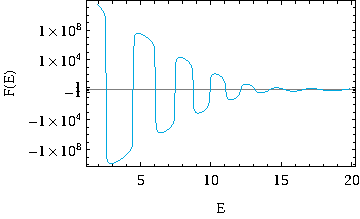
\includegraphics[scale = 1.388888888]{img/errorFunction.pdf}
	\caption{Fehlerfunktion für verschiedene Energien}
	\label{fig:shooting}
\end{figure}
In dieser Aufgabe sollte mit der Shooting Methode die Schrödingergleichung für ein lineares Potential $V(x\geq 0)=x$ gelöst werden. 
Dabei wurde von $x=\infty$, bzw. $\text{X\_MAX}=30$, bis $x=0$ mit der Numerov-Methode integriert.
Für die erste Randbedingung gilt $\psi(\infty\approx\text{X\_MAX})=0$, da das Potential unendlich ist.
Für die andere Seite gilt $\psi(0)=0$, da $V(x<0)=\infty$.
Damit diese erfüllt ist, muss die Fehlerfunktion $F(E) = \psi_E(0)$ eine Nullstelle haben.

In Abbildung \ref{fig:shooting} ist diese Fehlerfunktion gegen die Energie $E$ gezeichnet.
Die Daten wurden mit dem Program \ref{errorFkt} generiert.
\clearpage

Da die Fehlerfunktion stetig ist, wird in Program \ref{F_Bild} das Bisektions-Verfahren verwendet, um die Nullstellen zu finden.
Dies wird ausgehen von Schätzungen gemacht, die aus dem Abbildung \ref{fig:shooting} abgelesen wurden.
Nachdem das Intervall klein genug ist, wird die Wellenfunktion (im Array $\text{psi}$ gespeichert) normiert und abgespeichert.\\
Da dieser Prozess für alle Schätzungen gemacht werden muss wurde dies parallelisiert.

\begin{figure}
	\centering
	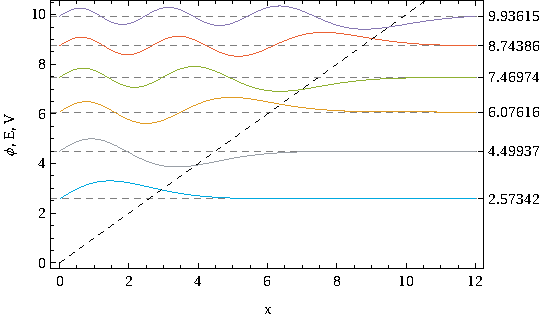
\includegraphics[scale = 1.388888888]{img/out.pdf}
	\caption{Potential mit verschiedenen Wellenfunktionen}
	\label{fig:out}
\end{figure}
In Abbildung \ref{fig:out} sind die so erhaltenen ersten 5 Wellenfunktionen und Energien dargestellt.\\s
Weitere 25 Wellenfunktionen sind in Abbildung \ref{fig:large} zu sehen. Die Eigenenergien sind in der Abbildung \ref{fig:trend} dargestellt.\smallskip

\clearpage
\begin{figure}
	\centering
	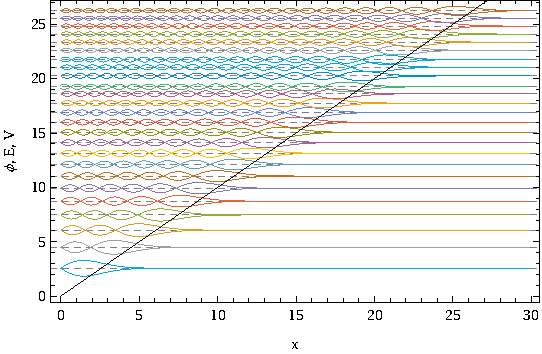
\includegraphics[scale = 1.388888888]{img/large.pdf}
	\caption{die ersten 25 Wellenfunktionen}
	\label{fig:large}
\end{figure}
\begin{figure}
	\centering
	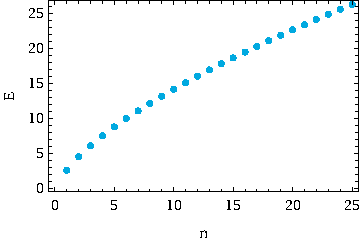
\includegraphics[scale = 1.388888888]{img/trend.pdf}
	\caption{Trend der Energieniveaus}
	\label{fig:trend}
\end{figure}


%%%%%%%%%%%%%%%%%%%%%%%%%%%% Code %%%%%%%%%%%%%%%%%%%%%%%%%%%%%%%%%%%
\clearpage
\section{Code}

\subsection*{6}
\lstinputlisting[label={errorFkt},caption={
	Programm zum berechnen der Error-Funktion für verschiedene Energien.
},language=c]{errorFkt.c}

\clearpage
\lstinputlisting[label={F_Bild},caption={
	Programm zum parallelisierten Berechnen der Wellenfunktionen mit der Shooting-;ethode.
},language=c]{schroedinger.c}

\end{document}
